\section{Data analysis}
\label{refl1:anal}
XRR and NR methods have a well documented history for the analysis of the structure of phospholipid monolayers at the air-water interface \cite{mohwald_phospholipid_1990,kewalramani_effects_2010,bayerl_specular_1990,johnson_structure_1991,clifton_role_2012,helm_phospholipid_1987,daillant_x-ray_1990}.
Typically these have involved using a model-dependent analysis method, however, the modelling approaches have varied significantly in the number of layers used, the shape of the layers, the use of interfacial roughness, the parameterisation of constraints employed, and even the method by which the reflectometry profile was calculated from the model.
Recently, an evaluation of the applicability of different models for surfactant and phospholipid monolayers using NR outlined a view of ``best practice'' \cite{campbell_structure_2018}.
However, frequently the constraints employed in the modelling process include the head and tail volume for the phospholipid head and tail groups.
These values are taken from a variety of other techniques, some examples are shown in Table~\ref{tab:water}.
%
\begin{sidewaystable}
    \centering
  \small
    \caption{Lipid component volumes extracted from different literature sources. $V_l$ corresponds to the total phospholipid volume, $V_t$ to the tail group volume, $V_h$ to the head group volume, MD to molecular dynamics simulations, WAXS to wide-angle X-ray scattering, NB to neutral buoyancy, and DVTD to differential vibrating tube densimetry.}
    \label{tab:water}
    \begin{tabular}{l | l l l | l l | l l | l | l}
        \toprule
        Phospholipid & \multicolumn{3}{l|}{DPPC} & \multicolumn{2}{|l|}{DMPC} & \multicolumn{2}{|l|}{DLPC} & DMPG & POPG \\
        \midrule
    Ref. & \cite{armen_phospholipid_1998} & \cite{sun_order_1994} & \cite{kucerka_determination_2004,balgavy_evaluation_2001}\footnote{The values for the head component in Ku\v{c}erka \emph{et al.} \cite{kucerka_determination_2004}, were taken from Balgav\'{y} \emph{et al}. \cite{balgavy_evaluation_2001}} & \cite{armen_phospholipid_1998} & \cite{kucerka_determination_2004,balgavy_evaluation_2001} & \cite{armen_phospholipid_1998} & \cite{kucerka_determination_2004,balgavy_evaluation_2001} & \cite{pan_molecular_2012} & \cite{kucerka_scattering_2012} \\
    \midrule
    $V_l$/\si{\angstrom\cubed} & \num{1287.3 \pm 25.5} & \num{1148 \pm 2} & \num{1268.2 \pm 32.1} & \num{1172.5 \pm 25.1} & \num{1155.4 \pm 30.0} & \num{1057.7 \pm 24.7} & \num{1046.6 \pm 28.0} & \num{1011.4} & \num{1203} \\
    $V_t$/\si{\angstrom\cubed} & \num{966.4 \pm 5.4} & \num{829 \pm 4} & \num{924.7 \pm 17.6} & \num{851.5 \pm 5.0} & \num{815.9 \pm 15.5} & \num{736.8 \pm 4.6} & \num{707.1 \pm 13.5} & \num{720.4} & \num{914} \\
    $V_h$/\si{\angstrom\cubed} & \num{320.9 \pm 20.1} & \num{319 \pm 6} & \num{339.5 \pm 14.5} & \num{320.9 \pm 20.1} & \num{339.5 \pm 14.5} & \num{320.9 \pm 20.1} & \num{339.5 \pm 14.5} & \num{291.0} & \num{289} \\
    \midrule
    Method & MD & WAXS & NB & MD & NB & MD & NB & DVTD & MD \\
    T/\si{\celsius}& 50 & 24 & 30 & 50 & 30 & 50 & 30 & 20 & 25 \\
        \bottomrule
    \end{tabular}
\end{sidewaystable}
%

Table~\ref{tab:water} provides a general consensus that the volume of the phosphocholine head group (PC) is \SIrange{320}{360}{\angstrom\cubed}, while the phosphatidylglycerol head group (PG) is \SIrange{289}{291}{\angstrom\cubed}.
However, these values were all determined from experiments or simulations where the head group was interacting with water molecules.
It is not clear if this will influence the volume that it occupies, and if that volume will change in the presence of a non-aqueous solvent, such as the DES considered herein.
The charged nature of the zwitterionic and anionic phospholipid head groups may have different interactions with the polar, but neutral water and the charged DES \cite{sanchez-fernandez_self-assembly_2018}.
Additionally, it is known that, on water, increased surface pressures and the associated Liquid-Expanded to Liquid-Condensed phase transition will lead to a compression of the phospholipid tail volume, compared to the values in Table~\ref{tab:water} \cite{marsh_molecular_2010,small_lateral_1984}, and that this compaction has not necessarily been accounted for in the literature \cite{campbell_structure_2018}.

These factors meant that it was necessary to develop a model that was considerate of the phospholipid chemistry while applying as much of the ``best practice'' from Campbell \emph{et al.} \cite{campbell_structure_2018} as possible, and ensuring that the head and tail group volumes were not constrained parameters.
The lack of having these normally constrained parameters meant that it was necessary to consider methods by which the reflectometry measurements could be co-refined, in a similar fashion to contrast variation co-refinement in neutron reflectometry.
This could be achieved by the co-refinement of reflectometry measurements at different surface pressures, as the model was considerate of the phospholipid chemistry, and the different surface pressures were in the same phase; Liquid-Condensed (LC) for DPPC and Liquid-Expanded (LE) for DMPC, DLPC, and DMPG.
Therefore the head and tail group volumes will remain constant, and only the surface concentration and normal tail thickness will vary.

The chemically-constrained model that has been used in this work was implemented in the Python library \texttt{refnx} \cite{nelson_refnx_2019,nelson_refnx_2019-1}.
The software enables the inclusion of custom model classes that feed parameters into the Abel\`{e}s model (Section~\ref{sec:refltheory}) \cite{abeles_sur_1948,parratt_surface_1954}.
Our chemically-consistent model class can be seen in Code Block~\ref{cb:chemconsis}, and is shared under a CC BY-SA 4.0 license in the ESI for the associated publication \cite{mccluskey_lipids_at_airdes_2019}.
In order to ensure that the phospholipid chemistry was consistent both within the phospholipid molecule and across the different surface pressures, Code Block~\ref{cb:const} was implemented.
%
\begin{figure}
    \centering
        \lstinputlisting[caption={The chemically-consistent model class that was implemented in \texttt{refnx} \cite{nelson_refnx_2019,nelson_refnx_2019-1}.},label={cb:chemconsis},firstline=1,lastline=72]{reports/code_blocks/mol_vol.py}
\end{figure}
%
\begin{figure}
    \centering
        \lstinputlisting[caption={The \texttt{set\_constraints} that was used to impose chemical-consistency on the phospholipid monolayer structure..},label={cb:const},firstline=5,lastline=22]{reports/code_blocks/ref_help.py}
\end{figure}
%

The chemically-consistent model, that is outlined in Code Block~\ref{cb:chemconsis}, consisted of two layers that define the phospholipid monolayer; the head layer at the interface with the solvent and the tail layer at the air interface.
The head groups have a scattering length that can be calculated from a summation of the X-ray or neutron atomic scattering lengths, $b_h$, and a volume, $V_h$.
These groups make up a layer of a given thickness, $d_h$, which has some interfacial roughness, $\sigma_h$, within which some volume fraction of solvent may penetrate, $\phi_h$.
The tail layer is defined in the same way, however, the tail thickness, $d_t$, is constrained such that it can be no greater than the maximum extended length for the phospholipid tail (defined as the Tanford length, $t_t$ \cite{tanford_hydrophobic_1980}), which is given in Table~\ref{tab:invar}, and that no solvent may penetrate into the layer (e.g. $\phi_t=0$).
Therefore, the $\text{SLD}$ may be determined as discussed in Equation~\ref{equ:sld}.
Based on the work of Campbell \emph{et al.} \cite{campbell_structure_2018}, a single value for the interfacial roughness was fitted for all of the interfaces, including the subphase (i.e. $\sigma_t = \sigma_h = \sigma_s$), as there is only a single phospholipid molecule type present in each monolayer.
Therefore, any capillary wave roughness at the air-DES interface is carried monotonically through the layers. The interfacial roughness was constrained to be greater than \SI{3.3}{\angstrom}, in agreement with previous work \cite{sanchez-fernandez_micellization_2016}.
%
\begin{table}
    \centering
  \small
    \caption{The invarient parameters within the chemically-consistent model.}
    \label{tab:invar}
    \begin{tabular}{l | l l l | l}
        \toprule
        Component & $b_t$/\si{\femto\meter} & $b_h$/\si{\femto\meter} & $t_t$/\AA & $\text{SLD}$/$10^{-6}$ \AA$^{-2}$ \\
        \midrule
    X-ray & & & & \\
        DPPC & 6827 & 4635 & 20.5\tablefootnote{\label{note:tanford}Values obtained from the Tanford formula \cite{tanford_hydrophobic_1980}.} & -- \\
        DMPC & 5924 & 4635 & 18.0\footref{note:tanford} & -- \\
        DLPC & 5021 & 4635 & 15.5\footref{note:tanford} & -- \\
        DMPG & 5924 & 4694 & 18.0\footref{note:tanford} & -- \\
        Air & -- & -- & -- & 0 \\
        DES & -- & -- & -- & 10.8\tablefootnote{\label{note:san}Values obtained from Sanchez-Fernandez \emph{et al.} \cite{sanchez-fernandez_micellization_2016}.} \\
        \midrule
        Neutron & & & & \\
        d$_{54}$-DMPC & & & 18.0\footref{note:tanford} & -- \\
        d$_{62}$-DPPC & & & 20.5\footref{note:tanford} & -- \\
        h-DES & -- & -- & -- & 0.43\footref{note:san} \\
        hd-DES & -- & -- & -- & 3.15\footref{note:san} \\
        \bottomrule
    \end{tabular}
\end{table}
%

The constraints implemented in Code Block~\ref{cb:const} involved two aspects.
The first was to ensure that the number density of head groups and pairs of tail groups was kept the same.
This was achieved with the following relation \cite{braun_polymers_2017},
%
\begin{equation}
\phi_h = 1 - \bigg(\frac{d_tV_h}{V_td_h}\bigg).
\label{equ:phih}
\end{equation}
%
The second aspect was to enforce chemically-consistant constraints across the measurements that were conducted at different surface pressures.
This was achieved by constraining the head and tail group volumes and the head layer thickness such that they do not vary between the different surface pressure measurements.

The justification for constraining the tail volume is built on the assumption that the phospholipids remain in the same phase.
On water, this may be demonstrated with a Langmuir isotherm.
However, it was not possible to collect consistent Langmuir isotherm measurements, due to the high viscosity of the DES.
Instead, grazing incidence X-ray diffraction was used to confirm the phases of DMPC and DPPC at \SI{30}{\milli\newton\per\meter}.
Figure~\ref{fig:gixd} shows the GIXD data from different phospholipids at different temperatures.
Unfortunately, all the patterns show a weak artefact due to scattering from the Teflon trough.
However, there are clear (2, 0) diffraction peaks in the GIXD pattern for DPPC at \SI{22}{\celsius} and DMPC at \SI{7}{\celsius} indicating that both lipids are in the LC phase.
This peak was also present at other surface pressures (data not shown).
The peak position corresponded well with that found for DPPC in water \cite{watkins_structure_2009}.
DMPC at \SI{22}{\celsius} showed no evidence of a diffraction peak indicating the presence of the LE phase.
It was assumed that DLPC and DMPG were also in the LE phase as there is no reason for the phase behaviour of these systems to differ significantly from that of DMPC at room temperature.
%
\begin{figure}
    \centering
    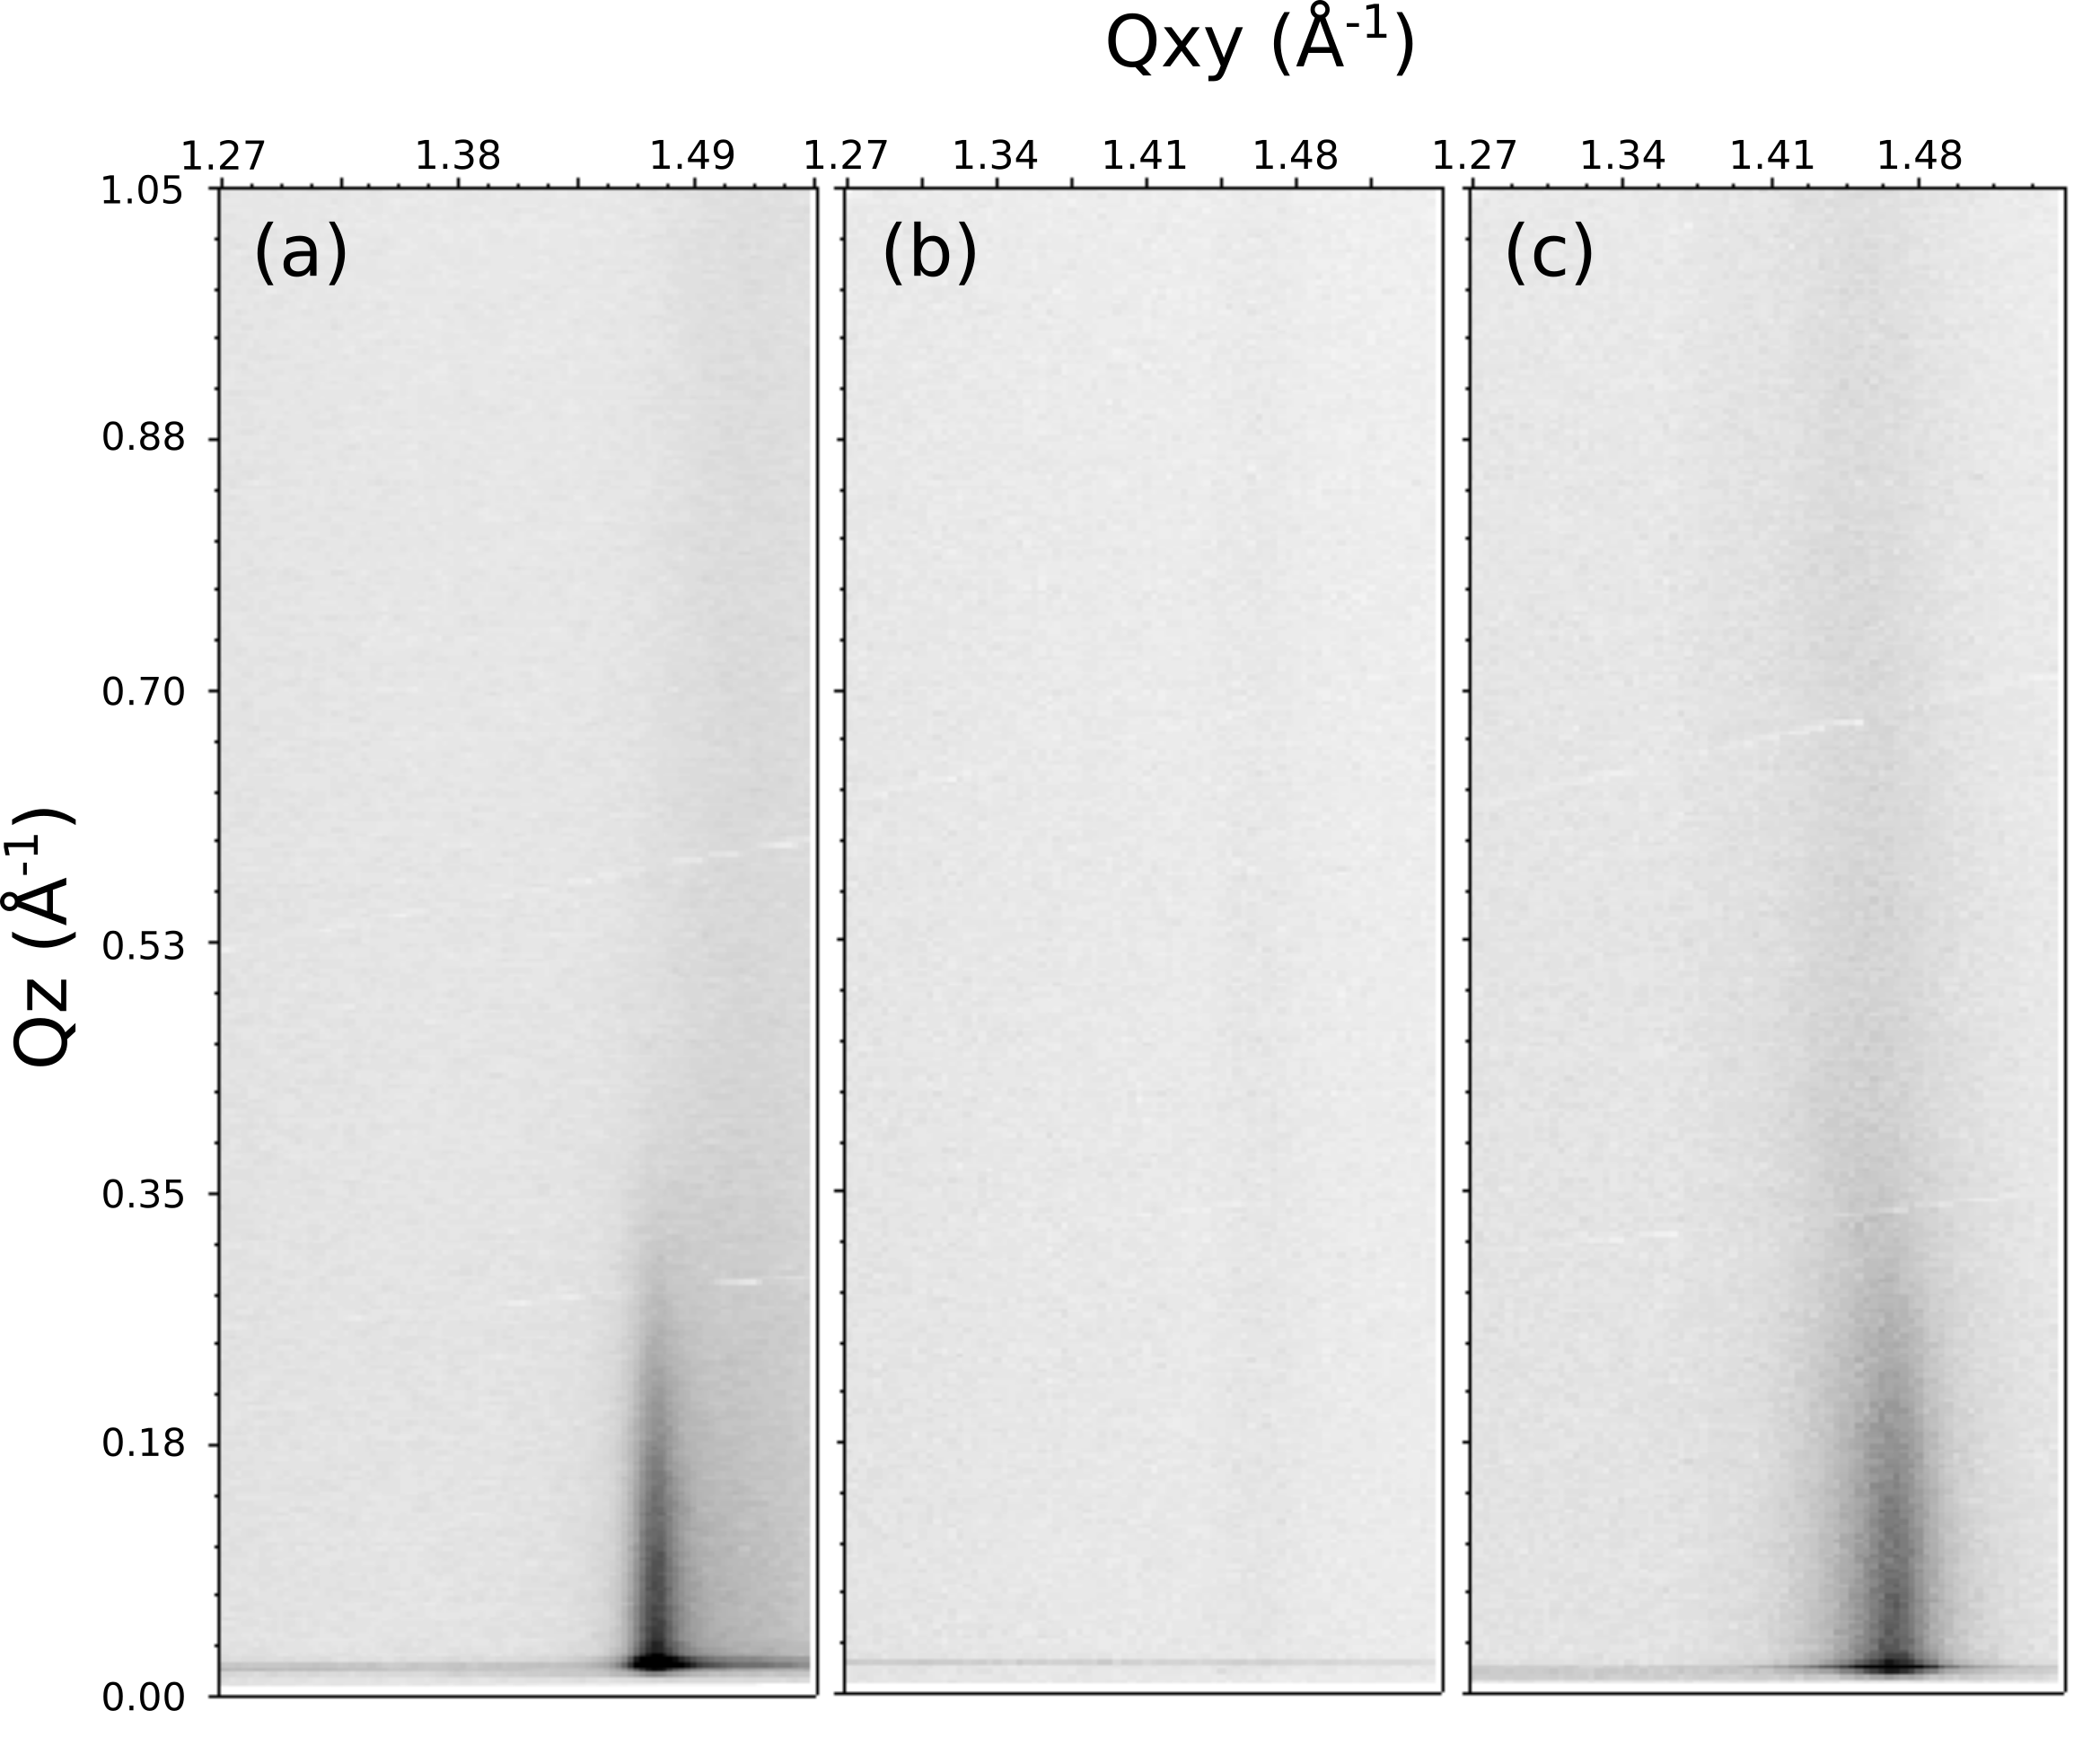
\includegraphics[width=0.6\textwidth]{reflectometry1/gixd}
    \caption{The GIXD patterns; (a) DPPC at \SI{30}{\milli\newton\per\meter} and \SI{22}{\celsius}, (b) DMPC at \SI{30}{\milli\newton\per\meter} and \SI{22}{\celsius}, and (c) DMPC at \SI{30}{\milli\newton\per\meter} and \SI{7}{\celsius}.}
    \label{fig:gixd}
\end{figure}
%

Initially, this chemically-consistent modelling approach was applied only to the XRR data.
The tail layer thickness and interfacial roughness were allowed to vary independently across the surface pressures, while the other parameters were constrained as discussed above or held constant to the values given in Table~\ref{tab:invar}.
For each co-refinement of four XRR measurements, there were, in total, eleven degrees of freedom.
Throughout all of the analyses, the intensity scale factor was allowed to vary freely, while the background was constrained to the intensity at the largest $q$-value.

Following this, the head and tail group volumes, and the head layer thickness that were found from the XRR analysis were used as fixed variables for the refinement of the NR measurements.
The reduced the number of fitted parameters in the NR data to two, namely the thickness of the tail layer, $d_t$, and the interfacial roughness, $\sigma_{t,h,s}$, for the co-refinement of two datasets.
Table~\ref{tab:invar} also presents details of the scattering lengths and SLDs using for the NR refinement.
Again, the intensity scale factor was allowed to vary freely and the background constrained to the intensity at the largest $q$-value.

In both the XRR and the NR analysis, the refinement of the chemically-consistent model to the experimental data involved the transformation of the reflectometry calculated from the model and the data into $Rq^4$-space, such that the contribution of the Fresnel decay was removed \cite{gerelli_aurore_2016}.
The model was then optimised using the differential evolution method that is available within the \texttt{scipy} library \cite{jones_scipy_nodate}.
This refined the parameters to give the best fit to the data.
Markov chain Monte Carlo (MCMC) was then used to probe the search-space available to each parameter, given the experimental uncertainty of the data.
The MCMC sampling method used was Goodman \& Weare's Affine Invarient Ensemble \cite{goodman_ensemble_2010} as impliemented in the \texttt{emcee} package \cite{foreman-mackey_emcee_2013}.
This enabled the determination of the probability distribution for each of the parameters, and therefore the quantification of their inverse uncertainty, given the uncertainty in the experimental data.
A Shapiro-Wilk test \cite{shapiro_analysis_1965} was used to determine the normality of each of the probability distribution functions (PDFs).
If the PDF failed the test the value was quoted with asymmetric confidence intervals, compared with the symmetric confidence intervals given for those that passed the Shapiro-Wilk test.
It is important to note that the PDFs and therefore the determined confidence intervals are not true confidence intervals, and account only for the uncertainty that is present in the data, i.e. they do not account for systematic uncertainty in the measurement technique.
In addition to determining parameter confidence intervals, it was also possible to use these probability distributions to understand the correlations present between the parameters and the impact this has on the fitting process.
The correlation was quantified using the Pearson correlation coefficient \cite{pearson_notes_1895}, a common statistical definition for the level of correlation present between two variables.
The Pearson correlation coefficient can have values that range from \numrange{-1}{1}, with a value of \num{-1} corresponding to a complete negative correlation (an increase in one variable is associated with a decrease in the other), while a value of \num{1} corresponds to a complete positive correlation (an increase in one variable is associated with a similar increase in the other), a value of \num{0} indicates no correlation between the two variables.
The MCMC sampling involved 200 walkers that were used for 1000 iterations, following a burn-in of 200 iterations.
